\chapter{スピン、アイソスピン、カラー、グルーオン自己相互作用}

\section{電気力学との類推による量子色力学}

量子色力学は一講義で完全に展開するにはあまりに広大な主題である。ここでの目的は、より深い数学ではなく、基本的な直観的描像である。

量子電気力学は電子と光子の理論である。それはまたクーロン力の量子論でもある。原子の原子核を、その運動や内部構造を問うことなく、電場の固定された源として扱うならば、QEDは原子の理論である。

量子色力学はクォークとグルーオンに対して同様の役割を果たす。それは粒子そのもの、粒子間の力、そしてそれらが形成する複合体を記述する。これらの複合体は\emph{ハドロン}と呼ばれる。陽子と中性子はバリオンである。すなわち、正味のクォーク数、あるいは同等に、非零のバリオン数を持つ。中間子はクォーク--反クォークの組み合わせである。バリオンと中間子のいずれもグルーオンを含む。

グルーオンは電気的に中性であるが、クォークを束縛する場を与える。その点でグルーオン場は、原子を束縛する電磁場に類似した役割を果たす。

カラーとグルーオンを導入する前に、スピンの数学に戻ると有用である。同じ数学がほとんどそのまま\emph{アイソスピン}として再び現れ、関連するパターンがカラーの理論においてもう一度現れる。群論がこれらの構成の下に横たわっているが、必要なアイデアは角運動量を通じて展開できる。

\section{角運動量多重項}

角運動量の成分は
\begin{equation}
[L_x,L_y]=i\hbar L_z,
\end{equation}
を満たし、巡回的な同伴関係
\begin{equation}
[L_y,L_z]=i\hbar L_x,
\qquad
[L_z,L_x]=i\hbar L_y.
\end{equation}
が成り立つ。3つの成分は可換でないため、それらすべてを同時に測定することはできない。したがって記述は1つの軸、慣例的に\(z\)軸を選び出し、その軸に沿った角運動量の成分によって状態をラベル付けする。

この選択は自然界における回転対称性を破らない。それは、記帳のために1つの方向を選ぶことによって、記述においてのみ対称性を破る。

\(z\)成分の許される値は量子化されており、\(\hbar\)の1単位ずつ異なる。これらの値を列挙する際に\(\hbar=1\)と置くと、スピン\(\ell\)の多重項は
\begin{equation}
m=\ell,\ell-1,\ldots,-\ell.
\end{equation}
を含む。したがって独立な状態の数は
\begin{equation}
2\ell+1.
\end{equation}
である。

最初のいくつかの多重項を明示的に書く価値がある。
\begin{align}
\ell=0:&\qquad m=0,\\
\ell=\frac12:&\qquad m=\frac12,-\frac12,\\
\ell=1:&\qquad m=1,0,-1,\\
\ell=\frac32:&\qquad
m=\frac32,\frac12,-\frac12,-\frac32,\\
\ell=2:&\qquad m=2,1,0,-1,-2.
\end{align}

当面の目的では、半整数スピンはフェルミオンに属し、整数スピンはボソンに属する。電子はスピン\(\tfrac12\)の粒子である。スピン零の粒子は角運動量を全く持たない。光子はスピン1を持ち、スピン1の状態は原子や原子核に対しても現れる。原子や原子核は同様にスピン\(\tfrac32\)を持つこともでき、同じ数え方がより高いスピンへと続く。

記法は全スピンとその成分を区別しなければならない。数\(\ell\)は多重項をラベル付けし、同時に可能な最大の\(z\)成分でもある。数\(m\)はその多重項内の特定の状態をラベル付けする。したがってスピン1の対象は3つの状態を持つのに対し、スピン\(\tfrac12\)の対象は2つを持つ。

\section{2つのスピン半整数粒子の合成}

2つのスピン\(\tfrac12\)粒子を考え、それらの軌道角運動量を無視する。それらのスピン積空間は4つの基底状態を含む。
\begin{equation}
|\uparrow\uparrow\rangle,\qquad
|\uparrow\downarrow\rangle,\qquad
|\downarrow\uparrow\rangle,\qquad
|\downarrow\downarrow\rangle.
\end{equation}
対応する\(z\)成分は
\begin{align}
|\uparrow\uparrow\rangle &: m=+1,\\
|\uparrow\downarrow\rangle &: m=0,\\
|\downarrow\uparrow\rangle &: m=0,\\
|\downarrow\downarrow\rangle &: m=-1.
\end{align}
である。

両方のスピンが上を向いた状態は、スピン1の多重項が必ず現れることを証明する。最大の\(z\)成分は\(+1\)である。スピン1の多重項は3つの状態
\begin{equation}
m=+1,\quad 0,\quad -1.
\end{equation}
のみを持つ。しかし積空間は4つの状態を含み、その中には\(m=0\)を持つ2つの独立な状態が含まれる。それらすべてが単一のスピン1多重項に属することはできない。余分な状態はスピン2ではありえない。スピン2の多重項は5つの状態を必要とするからである。したがって4つの積状態は、スピン1の3つの状態とスピン零の1つの状態に分かれなければならない。

2つの\(m=0\)基底状態のどの組み合わせがスピン1多重項に属するか。2つの粒子を交換する。揃った状態は変わらない。
\begin{equation}
|\uparrow\uparrow\rangle\longrightarrow|\uparrow\uparrow\rangle,
\qquad
|\downarrow\downarrow\rangle\longrightarrow|\downarrow\downarrow\rangle.
\end{equation}
対照的に、混合した積状態は交換される。
\begin{equation}
|\uparrow\downarrow\rangle
\longleftrightarrow
|\downarrow\uparrow\rangle.
\end{equation}
それらの和は交換の下で対称である。
\begin{equation}
|\uparrow\downarrow\rangle+|\downarrow\uparrow\rangle.
\end{equation}
規格化により\(1/\sqrt2\)の因子が与えられる。
\begin{equation}
|1,0\rangle
=
\frac{|\uparrow\downarrow\rangle
      +|\downarrow\uparrow\rangle}{\sqrt2}.
\end{equation}

\begin{figure}[h]
\centering
\includegraphics[width=0.78\textwidth]{lecture_02_figure_02.png}
\caption{スピン1三重項の\(m=0\)メンバーを形成する対称な混合スピン組み合わせ。}
\lectureframe{00:15:08}
\end{figure}

2つの揃った状態とともに、これによりスピン1三重項が与えられる。
\begin{align}
|1,+1\rangle &=|\uparrow\uparrow\rangle,\\
|1,0\rangle &=
\frac{|\uparrow\downarrow\rangle
      +|\downarrow\uparrow\rangle}{\sqrt2},\\
|1,-1\rangle &=|\downarrow\downarrow\rangle.
\end{align}
残りの直交する組み合わせは負符号を持つ。
\begin{equation}
|0,0\rangle
=
\frac{|\uparrow\downarrow\rangle
      -|\downarrow\uparrow\rangle}{\sqrt2}.
\end{equation}
それは交換の下で反対称であり、1状態のスピン零多重項を形成する。したがって
\begin{equation}
\frac12\otimes\frac12=1\oplus0.
\end{equation}

対称な混合スピン状態は\(m=0\)をもつが、\emph{全角運動量がゼロ}ではない。これはスピン1の三重項に属する。座標軸を回転させると、この状態は\(m=\pm1\)状態と混合する。反対称な組み合わせだけが\(\ell=0\)をもつ。

角運動量に関する限り、一重項は空っぽの空間のようなものである。エネルギー、電荷、その他の量子数をもつことはあるが、角運動量はもたない。

この区別は思考実験によって検証できる。角運動量の保存以外のすべての保存則を無視し、どの2粒子スピン状態が単純に消滅しうるかを問う。どちらの整列状態も消滅しえない。それぞれがスピン1の多重項に属するからである。対称な\(m=0\)状態もまた消滅しえない。その\(z\)成分はゼロであるが、全スピンは依然として1であり、他の軸に対して非自明な成分をもつ。反対称な一重項だけが、角運動量の保存に反することなく消滅しうる。

\begin{classroomqa}
\audiencequestion{対称な混合スピン状態を\(z\)軸に沿って測定すると、\(+1\)または\(-1\)が得られるか。\lecturetimestamp{00:19:28}}
\lecturerresponse{いいえ。\(z\)軸に沿ってはゼロが得られる。それでもこの状態は全スピン1をもつので、別の軸に沿った測定では\(+1\)または\(-1\)が得られうる。}
\end{classroomqa}

\section{3つのスピン半粒子}

次に3つのスピン\(\tfrac12\)粒子を組み合わせる。
\begin{equation}
2\times2\times2=8
\end{equation}
個の積状態がある。3つのスピンがすべて上を向いていれば、全\(z\)成分は\(+\tfrac32\)である。したがってスピン\(\tfrac32\)の多重項が存在しなければならない。それは
\begin{equation}
2\left(\frac32\right)+1=4
\end{equation}
個の状態を含む。

4つの状態が残る。それらは第2のスピン\(\tfrac32\)多重項を形成しえない。\(m=\pm\tfrac32\)をもつ状態はすでに使われているからである。残りの状態の最大成分は\(+\tfrac12\)と\(-\tfrac12\)だけである。また、3つの半整数スピンが全スピンゼロをつくることもできない。残りの状態はスピン\(\tfrac12\)多重項を形成しなければならない。

スピン\(\tfrac12\)多重項は2つの状態を含む。4つの状態が残っているので、2つの異なるスピン\(\tfrac12\)多重項が存在する：
\begin{equation}
\frac12\otimes\frac12\otimes\frac12
=
\frac32\oplus\frac12\oplus\frac12.
\end{equation}
このパターンは、スピン上およびスピン下と呼ばれる2つの状態が、アップおよびダウンと呼ばれる2つのクォークフレーバーに置き換えられると再び現れる。

\section{内部スピンとしてのアイソスピン}

アイソスピン、すなわち同位体スピンは、通常のスピンの内部的な類似物である。通常のスピンは物理空間の回転に結びついている。アイソスピンはそうではない。それは内部的な数学空間における変換に関わり、その2つの基本状態は
\begin{equation}
u,\qquad d.
\end{equation}
と同一視される。ここで\emph{アップ}および\emph{ダウン}という用語は単なるフレーバーラベルである。通常空間で上や下を指すものは何もない。

\editorialnote{内部スピン空間の定義とそれに続くハドロン質量スケールの議論との間の短い移行部分は、確信をもって復元できない。そこから追加の物理的主張は推論されない。}

なぜ\(u\)と\(d\)がこの類推に適しているのか。ハドロン物理の自然なエネルギー尺度は数百MeVである。典型的な軽い中間子は数百MeVの質量をもち、3つのクォークを核子に束縛するエネルギーも同様にその尺度にある。それに比べて、通常の原子核の束縛エネルギーはわずか数MeVである。したがって、原子核内で陽子と中性子を結びつけている力は、ハドロン内でクォークを束縛している力学よりもはるかに小さいエネルギー尺度で考えられている。

6つのクォークフレーバーのうち、\(u\)と\(d\)はハドロン尺度に比べて軽い。重いクォークは生成により多くのエネルギーを要し、それらを含むハドロンはより軽いものへ崩壊しうる。その結果、最も安定な軽いハドロンはアップクォークとダウンクォークからできている。

ダウンクォークはアップクォークより重く、ここで用いている推定ではおよそ2倍であるが、どちらの質量も数百MeVに比べれば小さい。第一近似では、両方ともハドロン尺度ではほぼ質量ゼロとして扱ってよい。さらに重要なことに、両者はほぼ等しい質量として扱ってよい。

この近似的な等しさは対称性をもたらす。アップクォークとダウンクォークを入れ替えても、強い相互作用の物理はほとんど変わらない。陽子
\begin{equation}
p\sim uud,
\end{equation}
と中性子
\begin{equation}
n\sim udd,
\end{equation}
が最も単純な例を与える。それらは\(u\)と\(d\)を交換することによって異なり、その質量は非常に近い。

したがって入れ替え
\begin{equation}
u\longleftrightarrow d
\end{equation}
は数学的に
\begin{equation}
|\uparrow\rangle\longleftrightarrow|\downarrow\rangle.
\end{equation}
のように扱われる。通常のスピンでは、この変換は空間における軸の回転に対応する。アイソスピンでは、それは内部空間における回転である。物理的意味は異なるが、数学は類似している。

\begin{figure}[h]
\centering
\includegraphics[width=0.80\textwidth]{lecture_02_figure_03.png}
\caption{2つのスピン\(\tfrac12\)状態の三重項・一重項分解。対応するアイソスピン構成の模型である。}
\lectureframe{00:27:42}
\end{figure}

接頭辞\emph{iso}は\emph{isotope}に由来する。古い核の記述では、陽子と中性子は1つの内部二重項の2つの成員とみなされていた。核内で陽子と中性子を入れ替えると、1つの同位体が別の同位体に変わる。クォーク模型は後に、この陽子-中性子の入れ替えを、根底にある\(u\)と\(d\)の入れ替えに帰着させた。

\begin{classroomqa}
\audiencequestion{アイソスピンはクォーク模型より先に存在したのか。\lecturetimestamp{00:30:19}}
\lecturerresponse{はい。アイソスピンはクォークより前に導入され、歴史的にはハイゼンベルクと結びついている。クォーク模型は後に、その\(u\)および\(d\)フレーバー的解釈を与えた。}
\end{classroomqa}

アイソスピンは自然界の厳密な対称性ではない。アップクォークとダウンクォークの質量は厳密には等しくなく、またそれらは異なる電荷をもつ：
\begin{equation}
Q(u)=+\frac23,
\qquad
Q(d)=-\frac13.
\end{equation}
たとえ質量が等しくても、電磁気学は依然として両者を区別するであろう。

小さなハドロン系および核系では、電磁気的効果は強い相互作用に比べて弱い。大きな原子核では電気的反発が重要になり得るが、陽子、中性子、あるいはヘリウムのような小さな原子核では、強い相互作用のスケールに対する比較的小さな補正である。したがってアイソスピン近似は2つの段階からなる：

\begin{enumerate}
\item \(u\)--\(d\)質量差を無視する；
\item それらの電磁気的区別を切り、強い相互作用のみを保持する。
\end{enumerate}

この近似の範囲内で、\(u\)と\(d\)の間の変換は、通常のスピン対称性と数学的に類似した対称性となる。

\section{核子アイソスピン二重項}

単一のクォークを孤立させ、自由な実験室の対象として調べることはできない。観測される最も単純なバリオンは3つのクォークを含む。したがって3スピンの数え上げの議論には、直接的なアイソスピンの類似物がある：3つのアイソスピン\(\tfrac12\)クォークは全アイソスピン\(\tfrac32\)または\(\tfrac12\)を形成し得る。

全アイソスピン\(\tfrac12\)から始める。そのような多重項は
\begin{equation}
2\left(\frac12\right)+1=2
\end{equation}
個の状態をもつ。それらは陽子と中性子である：
\begin{equation}
p\sim uud,
\qquad
n\sim udd.
\end{equation}
それらの電荷は
\begin{align}
Q(p)
&=\frac23+\frac23-\frac13
=+1,\\
Q(n)
&=\frac23-\frac13-\frac13
=0.
\end{align}
\(u\)と\(d\)を入れ替えると、陽子と中性子が入れ替わる。それらはアイソスピン\(\tfrac12\)二重項を形成する。

交換対称性を議論するために、暫定的に3つのクォークのスロットを\(1,2,3\)でラベルする。これらのラベルは固定されたクォークの位置と誤解されるべきではない；クォークは運動する。模式的な陽子因子は
\begin{equation}
d_1\bigl(u_2u_3-u_3u_2\bigr).
\end{equation}

\begin{figure}[h]
\centering
\includegraphics[width=0.58\textwidth]{lecture_02_figure_04.png}
\caption{模式的な陽子状態における反対称化された2つの\(u\)クォーク因子。}
\lectureframe{00:35:43}
\end{figure}

この表式の目的は、フェルミオン的交換反対称性を強調することである。それは完全な陽子波動関数ではない。完全な状態はフレーバー、通常のスピン、空間依存性、および---まもなく本質的となる---カラーを組み合わせなければならない。

\editorialnote{添字は暫定的なスロットまたは一粒子ラベルである。2つの同一な\(u\)フレーバー状態は通常の反対称アイソスピン一重項を形成しないので、表示された因子それ自体はアイソスピンゼロの結論を支持しない。それは局所的なスロット反対称化の段階としてのみ保持され；陽子の全アイソスピンはその完全な3クォーク状態から従う。}

先のスピン構成との限られた比較は、量子状態がラベルの交換の下で対称的または反対称的に結合され得ることである。その比較だけでは、表示された\(uu\)因子が担うアイソスピンを決定しない。

陽子は通常のスピン\(\tfrac12\)とアイソスピン\(\tfrac12\)の両方をもつ。中性子についても同様である。これらは異なる量子数である：通常のスピンは物理的回転に関わり、アイソスピンは\(u\)--\(d\)内部対称性に関わる。

\section{デルタ四重項}

3つの軽いクォークは全アイソスピン\(\tfrac32\)も形成し得る。結果として得られる4状態多重項はデルタ四重項である：
\begin{equation}
\begin{aligned}
\Delta^{++}&\sim uuu,
&
\Delta^{+}&\sim uud,
\\
\Delta^{0}&\sim udd,
&
\Delta^{-}&\sim ddd.
\end{aligned}
\end{equation}
デルタ状態はアイソスピン\(\tfrac32\)だけでなく通常のスピン\(\tfrac32\)をもつ。最大成分をもつ状態では、3つの通常のスピンが揃い、3つのアイソスピンが揃う。

\(uud\)のような組成だけでは、その状態が陽子であるか\(\Delta^+\)であるかを決定しない。同じフレーバー内容を異なる全スピン状態および全アイソスピン状態に結合することができる。

\begin{classroomqa}
\audiencequestion{デルタ四重項の\(uud\)成員を陽子から区別するものは何か。\lecturetimestamp{00:41:08}}
\lecturerresponse{それらの通常のスピンが異なる。陽子はスピン\(\tfrac12\)をもつのに対し、デルタ状態はスピン\(\tfrac32\)をもつ。クォークはまた異なる全アイソスピン状態に結合されている。}
\end{classroomqa}

\begin{classroomqa}
\audiencequestion{デルタ四重項の中間の成員はアイソスピン\(\tfrac12\)の状態か。\lecturetimestamp{00:41:52}}
\lecturerresponse{いいえ。それらのアイソスピン成分は\(+\tfrac12\)と\(-\tfrac12\)であるが、全アイソスピンは\(\tfrac32\)である。全アイソスピン\(\tfrac32\)の多重項は必然的に4つの成分状態を含む。}
\end{classroomqa}

4つのアイソスピン成分は
\begin{equation}
I_3=\frac32,\frac12,-\frac12,-\frac32.
\end{equation}
に対応する。それらの電荷は
\begin{align}
Q(\Delta^{++})&=+2,\\
Q(\Delta^{+})&=+1,\\
Q(\Delta^{0})&=0,\\
Q(\Delta^{-})&=-1.
\end{align}
である。中間の2つの電荷はたまたま陽子と中性子の電荷に等しいが、スピンとアイソスピンの結合の仕方が異なるため、状態は依然として区別される。

近似的なアイソスピン対称性により、4つのデルタの質量はほぼ等しくなる。小さな\(u\)--\(d\)質量差は四重項内に小さな分裂を生むだけである。共通のデルタ質量スケールはおよそ
\begin{equation}
m_\Delta\sim1200\,\mathrm{MeV},
\end{equation}
であるのに対し、陽子と中性子はおよそ
\begin{equation}
m_N\sim940\,\mathrm{MeV}.
\end{equation}
である。

\subsection{\texorpdfstring{\(\Delta^{++}\)}{Delta++}の崩壊}

デルタ状態は核子とパイ中間子に崩壊するのに十分な質量を持つ。次を考える：
\begin{equation}
\Delta^{++}\sim uuu.
\end{equation}
構成子が離れるにつれて、クォーク--反クォーク対が生成されうる。\(u\bar u\)の挿入を試みると最終状態に3つの\(u\)からなるバリオンが残り、利用可能なエネルギーでより軽い許容チャネルを与えない。代わりに\(d\bar d\)対を生成すると、構成子は
\begin{equation}
uuu+d\bar d
\longrightarrow
uud+u\bar d.
\end{equation}
として再編成できる。最終的な2つの複合粒子は
\begin{equation}
uud=p,
\qquad
u\bar d=\pi^+,
\end{equation}
であるので、
\begin{equation}
\Delta^{++}\longrightarrow p+\pi^+.
\end{equation}

\begin{figure}[h]
\centering
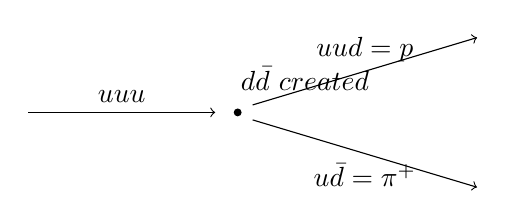
\begin{tikzpicture}[scale=0.95]
\draw[->] (-3,0) -- (-0.5,0) node[midway,above] {$uuu$};
\fill (-0.2,0) circle (1.5pt);
\draw[->] (0,0.1) -- (3,1.0) node[midway,above] {$uud=p$};
\draw[->] (0,-0.1) -- (3,-1.0) node[midway,below] {$u\bar d=\pi^+$};
\node at (0.7,0.45) {$d\bar d\ \text{created}$};
\end{tikzpicture}
\caption{崩壊\(\Delta^{++}\rightarrow p+\pi^+\)における構成子の再編成。}
\end{figure}

電荷の保存は直ちに成り立つ：
\begin{equation}
Q(p)+Q(\pi^+)=1+1=2=Q(\Delta^{++}).
\end{equation}
粗い質量バランスもこの崩壊を許す：
\begin{equation}
1200\,\mathrm{MeV}
>
940\,\mathrm{MeV}+140\,\mathrm{MeV}.
\end{equation}
最終状態の運動エネルギーに残るだけのエネルギーがある。

4つのデルタ状態はすべて、陽子または中性子とパイ中間子に崩壊しうる。それらの寿命は極めて短い。桁程度の見積もりは、光が陽子を横切るのにかかる時間である：
\begin{equation}
\tau_\Delta
\sim
\frac{10^{-13}\,\mathrm{cm}}
     {10^{10}\,\mathrm{cm/s}}
\sim10^{-23}\,\mathrm{s}.
\end{equation}
それでもなお、粒子衝突で生成される別個の物体として同定されるのに十分なほど長く生きる。

\begin{classroomqa}
\audiencequestion{この構成子の帳尻合わせにおいて、\(u\)と\(d\)の記号の書かれた順序は重要か。\lecturetimestamp{00:48:49}}
\lecturerresponse{当面の目的には重要でない。重要な情報はフレーバー内容と、完全な量子状態がどのように組み合わされるかである。}
\end{classroomqa}

\section{パウリのパズルとカラーの必要性}

\(\Delta^{++}\)は矛盾を露呈する。それは3つのアップクォークからなる。スピン\(\tfrac32\)の状態では、それらの通常のスピンはすべて同じ方向を向くことができる。それらはすべて\(u\)であるため、アイソスピンも同一である。スピン、フレーバー、および最低エネルギーの空間状態が記述のすべてであるならば、3つのクォークは同じ状態を占める同一のフェルミオンとなる。パウリの排他原理はこれを禁じる。

\begin{classroomqa}
\audiencequestion{繰り返されるアップクォークが同じ状態を占めるように見えるなら、どうしてフェルミオンでありうるのか。\lecturetimestamp{00:48:58}}
\lecturerresponse{それらはすべての量子数において同一ではありえない。\(\Delta^{++}\)は、クォークが通常のスピン、フレーバー、空間状態を超えた追加のラベルを必要とすることを示す。その追加のラベルがカラーである。}
\end{classroomqa}

新しいラベルには3つの可能な値がある：
\begin{equation}
r,\qquad g,\qquad b,
\end{equation}
赤、緑、青と呼ばれる。これらの語は可視光の色とは何の関係もない。それらは3つの内部状態に対する任意の名前である。他の名前を使うこともできたであろう。重要なのは、3つの異なる可能性が存在することである。

与えられたクォークフレーバーの赤、緑、青の版は、同じ質量と同じ通常の観測可能な性質を持つ。それでもなお、それらは異なる量子状態である。したがって\(\Delta^{++}\)は、1つの赤い\(u\)、1つの緑の\(u\)、1つの青い\(u\)を含むことができ、3つのフェルミオンは同じ完全な状態を占めない。

6つのフレーバーは
\begin{equation}
u,\ d,\ c,\ s,\ t,\ b.
\end{equation}
である。この順序は質量によるものではない。アップクォークが最も軽く、ダウンクォークが次に来る。チャームクォークはストレンジクォークよりずっと重く、トップクォークはボトムクォークよりはるかに重い。各フレーバーは3つのカラーで現れる。したがってクォークは少なくとも2つの異なる内部ラベルを担う：
\begin{equation}
\text{flavor}\quad\text{and}\quad\text{color}.
\end{equation}

代わりに3つのクォークを位置や運動量によって区別できたであろうか。デルタのパズルは最低エネルギー状態に関するものであり、その場合、関連する空間的・運動量的構造は、エネルギーと対称性の性質を変えずに3つの異なるラベルを与えることができない。欠けている区別は新しい内部自由度でなければならない。

原子物理学におけるスピンの役割との示唆に富む類推がある。同じ軌道状態を占めるように見える2つの電子でも、スピン状態によって異なりうる。同じ構造的な仕方で、フレーバー、通常のスピン、空間状態が一致するクォークは、カラーによって異なりうる。

\editorialnote{ヘリウム分光、パウリ原理、ウーレンベックとハウトスミットを含む正確な歴史的経路は、明示的に不確実なものとして扱われた。この類推は、これがスピンが発見された正確な年代順の経路であったと主張することなく、保持されている。}

南部陽一郎は、クォークがこの追加の自由度を必要とすることを認識したことに関連している。物理的な要点はその名称とは独立である。3つのクォークの色がパウリの矛盾を解決する。関連する排他原理はパウリ原理であり、ハイゼンベルクの不確定性原理ではない。

\editorialnote{名称\emph{color}の正確な帰属とその後の歴史は不確実なままにされたので、ここではより確固たる年代順は主張しない。ハイゼンベルクの不確定性原理への言及は、周囲のフェルミオン統計の議論が要求するように、パウリの排他原理へと訂正される。}

同じ色の構成が陽子と中性子にも当てはまる。それらの状態は、書かれた各フレーバー記号に永続的に識別可能な1つの色を割り当てることによって構築されるのではない。物理的なバリオンは、可能な赤、緑、青の割り当ての量子重ね合わせであり、適切な交換対称性と組み合わされている。

\begin{classroomqa}
\audiencequestion{色は直接測定できる通常の物理的性質なのか。\lecturetimestamp{00:56:55}}
\lecturerresponse{3つの色は同じ質量と同じ通常の性質をもつ。それらの区別は、許される組み合わせと衝突過程を通じて、関係的に明らかになる。実験は、孤立した色をもつクォークを直接検査のために用意することはできないにもかかわらず、3つの異なる色状態が存在することを示している。}
\end{classroomqa}

\begin{classroomqa}
\audiencequestion{色は保存されるのか。\lecturetimestamp{00:57:38}}
\lecturerresponse{はい。色は保存されるが、ここで議論している観測可能な粒子は常にゼロの色をもつので、やや珍しい見かけの保存則である。}
\end{classroomqa}

\editorialnote{より正確には、漸近的なハドロンは色一重項である。``ゼロの色''という表現は、赤、緑、青を数値的に足し合わせて得られるアーベル的な正味の電荷ではない。}

\begin{classroomqa}
\audiencequestion{\(uud\)陽子それ自体は本当に3つの色すべてを必要とするのか。2つの\(u\)クォークを区別するだけで十分に思える。\lecturetimestamp{00:57:58}}
\lecturerresponse{その例は明らかに何らかの追加の区別を必要とするが、3という数を不可避にするものではない。3つのアップクォークが平行な通常のスピンと平行なアイソスピンをもつ\(\Delta^{++}\)は、3つの異なるラベルの必要性を曖昧さなく示す。}
\end{classroomqa}

これが、デルタがこれほど重要な役割を果たした理由である。陽子と中性子はより複雑なスピンとフレーバーの対称性をもつので、矛盾はそれらの波動関数の詳細によって覆い隠されうる。\(\Delta^{++}\)では、対立は即座に現れる：
\begin{equation}
uuu,\qquad
\uparrow\uparrow\uparrow,
\qquad
\text{one lowest spatial state}.
\end{equation}
新しい3値のラベルが必要である。3つの色状態の存在は、ハドロン衝突のデータによっても独立に確認されている。

対称性のラベルは、その代替が孤立して等価である場合でも意味をもちうる。選ばれた空間軸がなければ、2つのスピン方向は物理的に等価である。第2の物体が基準軸を提供し、それらの関係を明らかにしうる。同様に、陽子または中性子はアイソスピン空間の方向を選び、他の状態との比較が内部の向きが平行か反平行かを明らかにする。色はより微妙であるが、その物理的内容も同様に、目に見える着色ではなく、関係、相関、相互作用規則を通じて現れる。

代わりにパウリ原理を放棄することを想像することもできる。それには新しい数学的枠組みが必要であろう。通常の量子場の理論は粒子をフェルミオンまたはボソンに分類し、この問題を解決する確立された第三の選択肢を提供しない。QCDはクォークのフェルミオン的性質を保ち、色を導入する。

\begin{classroomqa}
\audiencequestion{パウリ原理が要求する隠れた区別に対応する観測量は何か。\lecturetimestamp{01:01:08}}
\lecturerresponse{その問いは、よく知られた位置、運動量、アイソスピンの観測量よりもはるかに微妙である。その完全な答えには色の力学のより多くの部分が必要であり、後回しにされる。}
\end{classroomqa}

\begin{classroomqa}
\audiencequestion{クォークのフェルミオン的性質はハドロンのスピン割り当てから推論されたのか。\lecturetimestamp{01:01:43}}
\lecturerresponse{はい。}
\end{classroomqa}

\editorialnote{先行する2つの聴衆からの質問の文言は一部不明瞭である。それらの主題と簡潔な応答は確かであるが、それ以上詳細な定式化は推論されない。}

\begin{classroomqa}
\audiencequestion{陽子の中の1つのクォークに特定の色をどのように対応付けることができるのか。\lecturetimestamp{01:01:55}}
\lecturerresponse{恒久的に同定可能な構成要素に固定した色を割り当てるのではない。陽子は許される赤・緑・青のすべての割り当ての量子重ね合わせであり、スピン・フレーバー・空間・色の因子は適切に対称化または反対称化されている。\(\Delta^{++}\) が有用なのは、その平行スピンとフレーバー構造が、完全な陽子波動関数を必要とせずに色の必要性を露わにするからである。}
\end{classroomqa}

色はQCDにとって電荷が電気力学にとってそうであるようなものである。すなわち、相互作用を支配する量子数である。QCDはハドロン衝突からの実験データを非常に正確に説明する。この枠組みの究極的な正当化は、その帰結が実験と一致することである。

\section{光子とグルーオン}

クォークはQCDのフェルミオン的物質粒子であり、この限られた点ではQEDにおける電子に類似している。それらを束縛するものは何か。

電気力学では、電子は電磁場の源である。粒子の言葉では、電子は光子を放出・吸収し、光子の交換が荷電粒子間に力を生む。クォークも同様にグルーオン場の源であり、グルーオンを放出・吸収することができる。

グルーオンはいくつかの重要な点で光子に似ている。それらは質量のないスピン1の粒子であり、光子のような偏極状態をもつ。それらの運動量と偏極は通常の力学的性質である。決定的な違いは、グルーオンが色の情報を運ぶため、互いに相互作用することである。

光子は電荷を運ばない。原始的なQEDのレベルでは、1つの光子が別の光子を放出することはなく、2本の光線は相互作用せずに互いを通り抜ける。電子ループを伴う非常に小さな高次の光子-光子相互作用は存在するが、これらは直接的な光子の自己結合ではなく二次的効果である。空乏な空間では、素朴なQEDの頂点は単に電子が光子を放出または吸収するものである。

\begin{figure}[h]
\centering
\begin{tikzpicture}[scale=1.0]
\draw[->] (-2,-1) -- (0,0);
\draw[->] (0,0) -- (2,-1);
\draw[smooth] plot coordinates {
(0,0) (0.16,0.27) (0.32,0.23) (0.48,0.52)
(0.64,0.48) (0.80,0.77) (0.96,0.73)
(1.12,1.02) (1.28,0.98) (1.44,1.27)
(1.60,1.23) (1.76,1.52)
};
\node at (-1.25,-0.75) {$e^-$};
\node at (1.25,-0.75) {$e^-$};
\node at (1.95,1.62) {$\gamma$};
\fill (0,0) circle (1.5pt);
\end{tikzpicture}
\caption{素朴なQEDの頂点：電子が光子を放出または吸収する。}
\end{figure}

フェルミオン線の向きを逆にすると、電子の解釈が陽電子の解釈に変わる。放出・吸収・交差した陽電子過程はすべて、この1つの頂点の再配列である。

帳簿付けのために、光子が電子--陽電子対のいくつかの性質をもつと見なすことができる。その対は電気的に中性であり、揃った電子と陽電子のスピンは全スピン1を形成しうる。必要なエネルギーと運動量を供給する外部相互作用があれば、光子は電子--陽電子対を生成することができる。これはいずれも、光子が文字通り電子と陽電子からできていることを意味しない。架空の対の描像はQED自体にはほとんど寄与しないが、その色の類似物はQCDで有用である。

\section{グルーオンの色--反色ラベル}

クォークの3つの色状態を列として表す：
\begin{equation}
q=
\begin{pmatrix}
r\\
g\\
b
\end{pmatrix}.
\end{equation}
対応する反クォークのラベルを行として表す：
\begin{equation}
\bar q=
\begin{pmatrix}
\bar r&\bar g&\bar b
\end{pmatrix}.
\end{equation}

グルーオンはクォーク--反クォーク束縛状態ではない。それにもかかわらず、その色の帳簿付けは、1つの色と1つの反色を運ぶかのように振る舞う。したがって可能なラベルは次のように並べることができる：
\begin{equation}
\begin{pmatrix}
r\bar r&r\bar g&r\bar b\\
g\bar r&g\bar g&g\bar b\\
b\bar r&b\bar g&b\bar b
\end{pmatrix}.
\end{equation}
一見すると、これは9つの組み合わせを与える。

\begin{classroomqa}
\audiencequestion{対角の色--反色の成分は区別できないのか。\lecturetimestamp{01:13:37}}
\lecturerresponse{単純にそうではない。対角成分は区別される。要点は、それらの和が独立な量子状態ではないということである。}
\end{classroomqa}

実際には独立なグルーオン状態は8つだけである。3つの対角ラベルは互いに単純に区別できないのではないが、特定の対角和
\begin{equation}
r\bar r+g\bar g+b\bar b
\end{equation}
はQCDの追加の独立なグルーオンを与えない。この減少のより深い説明は後回しにする。当面の色の流れの議論では、9つの見かけのラベルで作業し、1つの対角の組み合わせが欠けていることを覚えておくと有用である。

\section{クォーク--グルーオン頂点}

クォークはグルーオンを放出し、同じ色または異なる色のいずれかで現れることができる。クォークが色 \(a\) で入り、色 \(b\) で出るなら、放出されたグルーオンは帳簿付けのラベル \(a\bar b\) を運ぶ：
\begin{equation}
a\longrightarrow b+(a\bar b).
\end{equation}
例えば、
\begin{equation}
r\longrightarrow g+(r\bar g).
\end{equation}
赤の色線はグルーオンへと続き、緑の線は出ていくクォークを通り抜け、グルーオンの中で反緑の線へと反転する。

クォークは色を変える必要はない。同じ規則はまた
\begin{equation}
r\longrightarrow r+(r\bar r),
\end{equation}
または
\begin{equation}
r\longrightarrow b+(r\bar b).
\end{equation}
を許す。

\begin{figure}[h]
\centering
\begin{tikzpicture}[scale=1.0]
\draw[->] (-2,-0.8) -- (0,0) node[midway,above] {$r$};
\draw[->] (0,0) -- (2,0.9) node[midway,above] {$g$};
\draw[smooth] plot coordinates {
(0,0) (0.20,-0.23) (0.40,-0.17) (0.60,-0.46)
(0.80,-0.40) (1.00,-0.69) (1.20,-0.63)
(1.40,-0.92) (1.60,-0.86) (1.80,-1.15)
(2.00,-1.09)
};
\node at (2.35,-1.12) {$r\bar g$};
\fill (0,0) circle (1.5pt);
\end{tikzpicture}
\caption{赤クォークが \(r\bar g\) グルーオンを放出しながら緑になる。}
\end{figure}

これはQCDの原始的な構成要素の1つである。

\begin{classroomqa}
\audiencequestion{グルーオンはクォークが色を変えるときだけ放出され得るのか。\lecturetimestamp{01:17:15}}
\lecturerresponse{いいえ。出ていくクォークの色は同じでも異なってもよい。いずれの場合も、放出されたグルーオンの色--反色ラベルによって色の線は連続する。}
\end{classroomqa}

\section{三グルーオン頂点}

QCDには、QEDに初等的な類似物をもたない別の基本的相互作用がある。グルーオンは他のグルーオンと直接相互作用できる。

\(r\bar b\)グルーオンから始める。色の流れの言葉では、それは次のように分裂し得る。
\begin{equation}
r\bar b
\longrightarrow
r\bar g+g\bar b.
\end{equation}
赤線は\(r\bar g\)へ、反青線は\(g\bar b\)へ続き、緑-反緑の対は二つの出ていくグルーオンに加わる。これが三グルーオン頂点を与える。

\begin{figure}[h]
\centering
\begin{tikzpicture}[scale=1.0]
\draw[smooth] plot coordinates {
(-2,0) (-1.80,0.12) (-1.60,-0.02) (-1.40,0.12)
(-1.20,-0.02) (-1.00,0.12) (-0.80,-0.02)
(-0.60,0.12) (-0.40,-0.02) (-0.20,0.12) (0,0)
};
\draw[smooth] plot coordinates {
(0,0) (0.20,0.27) (0.40,0.21) (0.60,0.50)
(0.80,0.44) (1.00,0.73) (1.20,0.67)
(1.40,0.96) (1.60,0.90) (1.80,1.19) (2.00,1.13)
};
\draw[smooth] plot coordinates {
(0,0) (0.20,-0.27) (0.40,-0.21) (0.60,-0.50)
(0.80,-0.44) (1.00,-0.73) (1.20,-0.67)
(1.40,-0.96) (1.60,-0.90) (1.80,-1.19) (2.00,-1.13)
};
\node at (-2.45,0) {$r\bar b$};
\node at (2.45,1.18) {$r\bar g$};
\node at (2.45,-1.18) {$g\bar b$};
\fill (0,0) circle (1.5pt);
\end{tikzpicture}
\caption{三グルーオンの色の流れ：\(r\bar b\rightarrow r\bar g+g\bar b\)。}
\end{figure}

許されるすべての組み合わせを暗記する必要はない。図を通して各色線をたどればよい。フェルミオン線が時間方向を逆転するときは、対応する反粒子または反色線として読み替える。

\section{グルーオン交換と力}

グルーオンは、光子が荷電粒子の間で交換されることによって電磁気力を生じるのとちょうど同じように、交換されることによって力を生じる。

例えば、青クォークと反青反クォークは\(g\bar b\)グルーオンを交換して、緑と反緑として出てくることができる。両方の頂点を満たす色の流れの割り当ては\footnote{正味の色の変化\(b+\bar b\longrightarrow g+\bar g\)は明白であるが、局所的な色ラベルは何度か修正される。交換されるラベル\(g\bar b\)は、両方の頂点で連続した色の流れを要求することによって再構成される。}
\begin{equation}
b+\bar b
\longrightarrow
g+\bar g.
\end{equation}
反クォーク頂点では、
\begin{equation}
\bar b\longrightarrow\bar g+(g\bar b),
\end{equation}
一方、クォーク頂点では、
\begin{equation}
b+(g\bar b)\longrightarrow g.
\end{equation}
交換されるグルーオンは、色の変化を一方のフェルミオン線から他方へ運ぶ。

\begin{figure}[h]
\centering
\begin{tikzpicture}[scale=1.0]
\draw[->] (-1.8,0) -- (-1.8,-1.8) node[midway,left] {$\bar b$};
\draw[->] (-1.8,1.8) -- (-1.8,0) node[midway,left] {$\bar g$};
\draw[->] (1.8,-1.8) -- (1.8,0) node[midway,right] {$b$};
\draw[->] (1.8,0) -- (1.8,1.8) node[midway,right] {$g$};
\draw[smooth] plot coordinates {
(-1.8,0) (-1.50,0.13) (-1.20,-0.03) (-0.90,0.13)
(-0.60,-0.03) (-0.30,0.13) (0,-0.03)
(0.30,0.13) (0.60,-0.03) (0.90,0.13)
(1.20,-0.03) (1.50,0.13) (1.8,0)
};
\node at (0,0.42) {$g\bar b$};
\fill (-1.8,0) circle (1.5pt);
\fill (1.8,0) circle (1.5pt);
\end{tikzpicture}
\caption{\(g\bar b\)グルーオンの交換は、青--反青の対を緑--反緑の対に変える。反クォークの矢印は時間の増加と逆向きである。}
\end{figure}

同じ相互作用はグルーオン間の力も許す。一貫した実現は\footnote{講義はグルーオン間のグルーオン交換と線をたどる規則を確立するが、図中の局所ラベルは繰り返し改訂される。示された割り当ては、すべての中間ラベルの確実な転記というよりも、最終的な規則の一つの一貫した実現である。}
\begin{equation}
(r\bar b)+(b\bar r)
\longrightarrow
(r\bar g)+(g\bar r),
\end{equation}
であり、\(g\bar b\)グルーオンが二つの外部グルーオンの間で交換される：
\begin{align}
r\bar b&\longrightarrow r\bar g+g\bar b,\\
b\bar r+g\bar b&\longrightarrow g\bar r.
\end{align}

\begin{figure}[h]
\centering
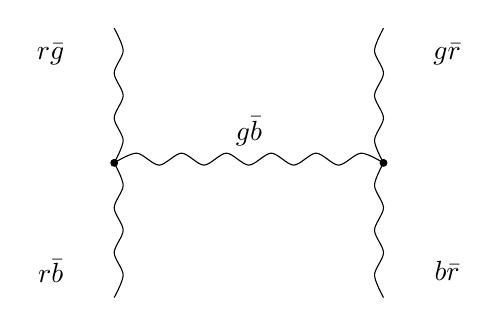
\begin{tikzpicture}[scale=0.95]
\draw[smooth] plot coordinates {
(-1.8,-1.8) (-1.68,-1.50) (-1.80,-1.20) (-1.68,-0.90)
(-1.80,-0.60) (-1.68,-0.30) (-1.8,0)
};
\draw[smooth] plot coordinates {
(-1.8,0) (-1.68,0.30) (-1.80,0.60) (-1.68,0.90)
(-1.80,1.20) (-1.68,1.50) (-1.8,1.8)
};
\draw[smooth] plot coordinates {
(1.8,-1.8) (1.68,-1.50) (1.80,-1.20) (1.68,-0.90)
(1.80,-0.60) (1.68,-0.30) (1.8,0)
};
\draw[smooth] plot coordinates {
(1.8,0) (1.68,0.30) (1.80,0.60) (1.68,0.90)
(1.80,1.20) (1.68,1.50) (1.8,1.8)
};
\draw[smooth] plot coordinates {
(-1.8,0) (-1.50,0.13) (-1.20,-0.03) (-0.90,0.13)
(-0.60,-0.03) (-0.30,0.13) (0,-0.03)
(0.30,0.13) (0.60,-0.03) (0.90,0.13)
(1.20,-0.03) (1.50,0.13) (1.8,0)
};
\node at (-2.65,-1.45) {$r\bar b$};
\node at (-2.65,1.45) {$r\bar g$};
\node at (2.65,-1.45) {$b\bar r$};
\node at (2.65,1.45) {$g\bar r$};
\node at (0,0.42) {$g\bar b$};
\fill (-1.8,0) circle (1.5pt);
\fill (1.8,0) circle (1.5pt);
\end{tikzpicture}
\caption{二つのグルーオン間の\(g\bar b\)グルーオンの交換。各色線と反色線は頂点を通して連続している。}
\end{figure}

\section{グルーオンの自己相互作用と非線形場}

グルーオンの自己相互作用はQCDの性格を変える。クォークはグルーオンを交換することによって束縛されてハドロンを形成し得るが、グルーオンもグルーオンを交換することによって束縛され得る。したがってQCDは、クォークをまったく含まず、グルーオン的自由度のみからなる複合物体を含み得る。QEDには、光子のみからなる対応する初等的束縛状態は存在しない。

場の言葉でも同じ結論が得られる。真空中の二つの電磁波は初等的なレベルでは互いを通り抜ける。二つのグルーオン波は相互作用し、互いを変形させる。一つのグルーオン場の配置の異なる部分同士でさえ、互いに力を及ぼし得る。したがってグルーオン場は非線形である。

\begin{classroomqa}
\audiencequestion{図の各側に同じ数の赤、緑、青のラベルが現れなければならないのか。\lecturetimestamp{01:24:59}}
\lecturerresponse{実際の規則は、図を通してすべての色線をたどることである。その連続性が色の保存である。フェルミオン線が時間的に向きを変えるなら、そのラベルは対応する反粒子または反色のラベルになる。}
\end{classroomqa}

\begin{classroomqa}
\audiencequestion{図の最初の版にあるすべての色ラベルと反色ラベルは一貫しているのか。\lecturetimestamp{01:26:00}}
\lecturerresponse{いいえ。いくつかのラベルは修正されなければならない。一貫した割り当てでは、赤、反青、緑の線がそれぞれ頂点を通して続き、逆向きのフェルミオン矢印は反粒子として解釈される。}
\end{classroomqa}

\begin{classroomqa}
\audiencequestion{中間グルーオン線はクォーク--反クォーク対として扱われているのか。\lecturetimestamp{01:27:58}}
\lecturerresponse{その色の帳簿付けにおいてのみである。グルーオンは文字通りにはクォーク--反クォークの複合体ではないが、対応する色と反色の性質を担っている。}
\end{classroomqa}

この段階では、初等的な規則は簡潔である：

\begin{itemize}
\item クォークはグルーオンを放出し吸収する；
\item グルーオンはグルーオンと直接相互作用する；
\item すべての色線と反色線は頂点を通して続かなければならない；
\item フェルミオン線を時間的に逆転させると、それは対応する反粒子線に変わる。
\end{itemize}

\begin{classroomqa}
\audiencequestion{これらすべての色--反色の線で表されるとき、グルーオンは依然として質量ゼロなのですか。\lecturetimestamp{01:28:13}}
\lecturerresponse{はい。グルーオンは依然として質量ゼロである。以下の限定は、ハドロン内部のクォークに割り当てられる質量が何を意味するかに関するものである。}
\end{classroomqa}

次に閉じ込めとハドロンの構造、すなわち孤立した色が決して観測されない理由と、クォークとグルーオンが複合粒子の内部でどのように組織化されるかを扱う。まず、構成子クォークの質量が何を意味するかを明確にしておくと有用である。

\section{プローブのスケールとクォーク質量の意味}

質量\(m\)の小さな物体が、柔らかく変形可能な材料の一片---ぶら下がったチューインガムで十分であるものに取り付けられていると想像しよう。非常にゆっくりと、柔らかい材料が調整する時間を持ち、系全体が一緒に動くように、ごく穏やかな力を加える。そのとき測定される慣性は、小さな物体の慣性に付随する材料の慣性を加えたものである。

次に、小さな物体を非常に高い振動数で揺さぶる。柔らかい材料は速い運動に追随する時間を持たない。ほぼ静止したままで、小さな芯が応答する。そのとき測定される高振動数の慣性は、\(m\)のみにはるかに近い。

\begin{figure}[h]
\centering
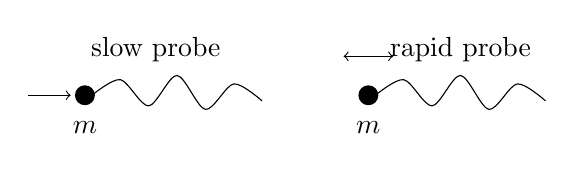
\begin{tikzpicture}[scale=0.9]
\fill (-3,0) circle (4pt);
\node at (-3,-0.45) {$m$};
\draw[smooth] plot coordinates {
(-2.9,0) (-2.5,0.22) (-2.1,-0.15) (-1.7,0.28)
(-1.3,-0.20) (-0.9,0.16) (-0.5,-0.08)
};
\draw[->] (-3.8,0) -- (-3.2,0);
\node at (-2.0,0.65) {slow probe};

\fill (1.0,0) circle (4pt);
\node at (1.0,-0.45) {$m$};
\draw[smooth] plot coordinates {
(1.1,0) (1.5,0.22) (1.9,-0.15) (2.3,0.28)
(2.7,-0.20) (3.1,0.16) (3.5,-0.08)
};
\draw[<->] (0.65,0.55) -- (1.35,0.55);
\node at (2.3,0.65) {rapid probe};
\end{tikzpicture}
\caption{遅いプローブは芯とその柔らかい付属物を一緒に動かすのに対し、速いプローブは主に芯の応答を測定する。}
\end{figure}

これは古典的な類推である。系の異なる部分が異なる振動数で参加する時間を持つため、推論される質量は加えられた力の振動数に依存する。

ハドロン内部のクォークは、強い相互作用をするグルーオン的な材料と他の構成要素に囲まれている。クォークを非常にゆっくり引くことができれば、ハドロン全体が応答するであろう。そのとき遭遇する慣性は核子の質量程度、
\begin{equation}
m_N\sim930\text{--}940\,\mathrm{MeV}.
\end{equation}
クォークが非常に強く叩かれ、非常に短い時間でプローブされれば、初期の応答は軽いクォークに慣習的に割り当てられるはるかに小さな質量パラメータ、ここで用いている見積もりではおよそ
\begin{equation}
m_{u,d}\sim5\text{--}10\,\mathrm{MeV}
\end{equation}
に関連する。

したがって「``クォークの質量''」という表現には、プローブのスケールの指定が必要である。穏やかな低振動数の擾乱は広がった複合体を動かし、強い高振動数の擾乱は最初により小さな部分を分解する。この類推は繰り込みの導出ではないが、粒子を記述するために用いられるパラメータが、それが測定される相互作用の振動数と波長に依存する理由を動機づける。このようなスケール依存のパラメータは走るパラメータまたは走る定数と呼ばれる。

\begin{classroomqa}
\audiencequestion{この振動数依存の質量は、\(\Delta x\,\Delta t\)のような不確定性関係の言い換えにすぎないのですか。\lecturetimestamp{01:33:32}}
\lecturerresponse{いいえ。この例はすでに古典的な現象である。柔らかいものに取り付けられた小さな質量は、速い力の下では一方の仕方で加速し、遅い力の下では別の仕方で加速する。それは、取り付けられた材料の異なる量が応答する時間を持つからである。}
\end{classroomqa}

\begin{classroomqa}
\audiencequestion{電子の電荷についての以前の議論も、同じ種類のスケール依存を含むのですか。\lecturetimestamp{01:34:04}}
\lecturerresponse{はい。一般的な教訓は、粒子を記述するために用いられるパラメータが、それがプローブされる相互作用の振動数と波長に依存するということである。それらは走る定数と呼ばれる。}
\end{classroomqa}

\begin{classroomqa}
\audiencequestion{クォークに割り当てられる分数電荷にも同じ限定が当てはまりますか。\lecturetimestamp{01:34:36}}
\lecturerresponse{当てはまる。クォークの電荷が何を意味するかを注意深く定義しなければならない。この段階では陽子の電荷に対して相対的に示されており、より完全な定義は別の議論である。}
\end{classroomqa}

\editorialnote{固定された分数電気電荷の量子数と、スケール依存の相互作用結合は別個のものである。結合の走りは\(+\tfrac23\)や\(-\tfrac13\)というフレーバーラベル自体を変えない。}

\begin{classroomqa}
\audiencequestion{なぜ色の帳簿付けは常にクォークと反クォークを用いるのですか。なぜ2つのクォークで対応する対象を作れないのですか。\lecturetimestamp{01:34:55}}
\lecturerresponse{それは重要な問いであるが、その答えは許される色の組み合わせと閉じ込めについての次の議論に属する。}
\end{classroomqa}

\begin{classroomqa}
\audiencequestion{個々のクォークを単離できないのなら、分数電荷、カラー、クォーク模型はどのようにして推論されたのですか。\lecturetimestamp{01:35:17}}
\lecturerresponse{その描像は、多くの手がかりと一見した矛盾がともに寄り集まって徐々に現れた。ハドロンのパターンはクォーク構成要素を示唆し、デルタ状態はフェルミ統計との衝突を露呈し、クォークの永久閉じ込めはさらに別の奇妙な事実をもたらした。クォークの提案は1960年代初頭に現れ、南部はカラーの着想の重要な初期版を持っており、多くの物理学者がほぼ続く十年の間に全構造を組み立てて検証した。それは一つの観測や一人の人物の結果ではなかった。}
\end{classroomqa}

\begin{classroomqa}
\audiencequestion{なぜ見かけ上のカラー--反カラーの組み合わせ9個ではなく、グルーオンは8個しかないのか。\lecturetimestamp{01:37:24}}
\lecturerresponse{対角和がなぜ追加のグルーオンではないのかの詳細な説明は後回しにする。}
\end{classroomqa}

\begin{classroomqa}
\audiencequestion{このQCDの議論は電子を無視しているのか。\lecturetimestamp{01:37:33}}
\lecturerresponse{はい。QCDは、QEDの議論が一時的にクォークを無視しうるのと同じ仕方で切り離されている。別々のセクターは最終的に、クォーク、電子、光子、その他の粒子を含むより大きな構造へと統合されなければならない。そのより大きな統合の一部は達成されており、一部は未完成のままである。物理学はしばしば、部分系を切り離し、それを理解し、それから断片を再び組み合わせることによって進む。}
\end{classroomqa}
